\documentclass[a4paper,twoside]{article}
\usepackage[hmarginratio=1:1,top=32mm,columnsep=20pt]{geometry} % custom page layout
\usepackage[T1]{fontenc}
\usepackage[utf8]{inputenc}
\usepackage[english]{babel}
\usepackage{lmodern}
\usepackage{fixltx2e} % \textsubscript command
\usepackage{soulutf8} % \ul command
\usepackage{changepage} % indentation (in title page)
\usepackage[font=it]{caption} % captions in italics
\usepackage[font=it]{subcaption} % subcaptions in italics
\usepackage{multicol}
\usepackage{cancel} % \cancel command
\usepackage{textcomp} % symbols
\usepackage{amsmath, amssymb}
\usepackage{amsthm}
\usepackage{makeidx}
\usepackage{graphicx}
\usepackage{float}
\usepackage{wrapfig}


\usepackage{verbatim}
\usepackage{listings}
\lstset{language=vhdl,%
	  keywordstyle=\color{Blue},
      basicstyle=\small\ttfamily,
      frame=TB,
      commentstyle=\color{red},
      showstringspaces=false
}
\usepackage[dvipsnames,usenames]{color}
\usepackage{fancyhdr}

%\usepackage{draftwatermark}
%\SetWatermarkText{Doc interno}



\pagestyle{fancy}
%\renewcommand{\chaptermark}[1]{\markboth{#1}{}}
\renewcommand{\sectionmark}[1]{\markright{ \thesection \space - \space #1}}
\renewcommand{\subsectionmark}[1]{\markright{\thesubsection \space - \space #1}}
\fancyhf{} \fancyhead[RO, LE]{\bfseries \thepage}
 \fancyhead[RE, LO]{
\includegraphics[scale=0.03]{Immagini/262}\bfseries}
\fancyhead[CO, CE]{\bfseries\rightmark}
%\fancyhead[CE]{\bfseries \leftmark}
\renewcommand{\headrulewidth}{0.5pt}
\renewcommand{\footrulewidth}{0pt}
\addtolength{\headheight}{0.5pt} \fancypagestyle{plain}{
\fancyhead{}
\renewcommand{\headrulewidth}{0pt}}

\newtheorem{thm}{Teorema}[section] 
\newtheorem{cor}[thm]{Corollario} 
\newtheorem{lem}[thm]{Lemma} 
\newtheorem{prop}[thm]{Proposizione} 
\theoremstyle{definition} 
\newtheorem{defn}{Definizione}[section]
\theoremstyle{remark} 
\newtheorem{oss}{Osservazione} 
\frenchspacing
\author{Alessandro Salvato}

\newcommand{\paginavuota}{\newpage\null\thispagestyle{empty}\newpage\null}

\begin{document}
\bibliographystyle{unsrt}
\thispagestyle{empty}
\begin{figure}[H]
\centering

\includegraphics[scale=.3]{Immagini/262}
\label{262}
\end{figure}
\begin{center}
\LARGE { \textbf {POLITECNICO DI TORINO} }\\ [1\baselineskip]
%Raccolta di Appunti \\ [2\baselineskip]
\huge{ \textbf{Electronics for Embedded Systems}}\\ [1\baselineskip]
\Huge{\textbf{Project of the course}}\\[1\baselineskip]


\end{center}

\begin{flushleft}
\large{Professor: Claudio Passerone}
\end{flushleft}
\begin{flushleft}
\large{Data: \today}
\end{flushleft}
\begin{flushleft}
\large{Author: Alessandro Salvato} 
\end{flushleft}


\clearpage
\paginavuota

\tableofcontents
\newpage

\section{Introduction}
I'm very glad to present by this report, my own project for Electronics for Embedded Systems course. The main idea consists in  realizing a camera able to capture photos to be transferred to an host computer for further processing. Before describing in details the environmental structure, I guess it's fundamental to highlight that all the topics of the course have been covered in the following manner:
\begin{itemize}
\item \textbf{Memory}: memory controller as FSM
\item \textbf{Programmable logic device}: acts as remote to send the user command
\item \textbf{Interconnection protocol}: I2C, SCCB and UART
\item \textbf{Peripheral management}: programming of camera peripheral
\item \textbf{AD and DA converters}: usage of AD converter to sample the luminance of the environment
\item \textbf{Power management}: Step-down converter to drive a LED
\end{itemize}
Each of them owns a proper section below.
\newline
Let's have a look on the general architecture, listing the main parts of the system. The camera is connected to an ST microcontroller: a STM32F446ZET. The choice on this MCU has due to the fact that it integrates a very useful and widespread engaged peripheral in the video-capturing field: the Digital CaMera Interface (\textbf{DCMI}). All images are sent to the host computer by UART protocol, exploiting another embedded peripheral of the microcontroller. Computer reads UART's data plugging a USB-UART adapter.  Then a small Python script converts those data into a BMP image. 
\newline
The command is generated by the user pushing a specific button. An 8 buttons keyboard is tied up to the FPGA: an Altera Cyclone IV on DE0-Nano board. The implemented VHDL is composed of the keyboard driver and a fully structural UART peripheral. When a button has clicked, an encoded 8-bit data is sent to the microcontroller, which, by an interrupt, recognizes that the user pushed something. 
\newline
A breadboard has been used to build circuits for AD and Bulk converters. For sure, the following image is more clarifying for the reader.
\newline
\newline
I used STM32 CubeIDE to program the microcontroller , a software Eclipse based. To program the FPGA I exploited both Quartus II when uploading the \textit{sof} file and Xilinx ISE Design Suite when simulating (just for my high familiarity with that). Moreover, as classical laboratory instruments I relied on an oscilloscope provided by GW Instek and a multimeter for resistor measurements.
\newline
\newline
Images captured are in the format QVGA
\begin{figure}[H]
\centering
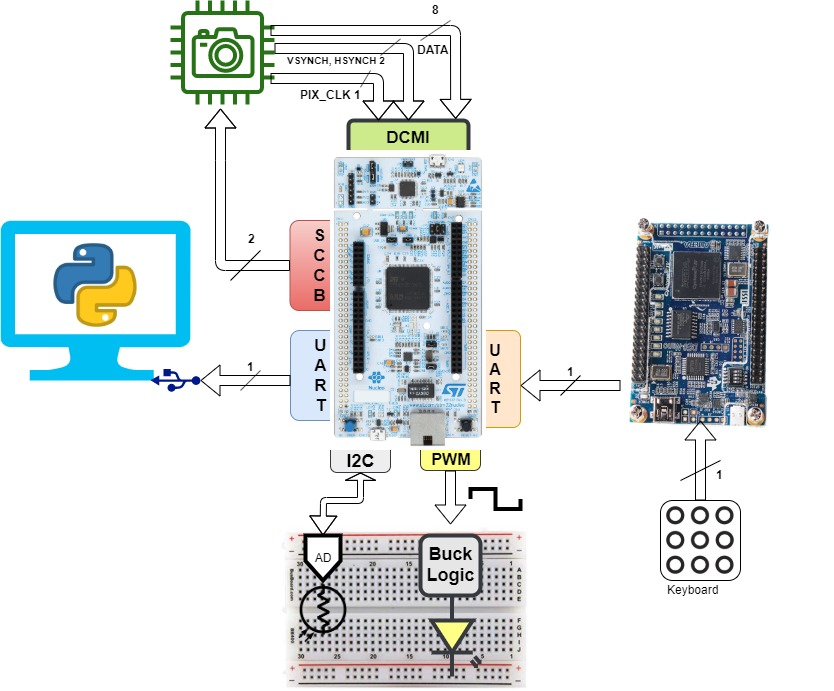
\includegraphics[scale=.5]{Immagini/01}
\label{01}
\caption{General block schema}
\end{figure}

What actually is

\begin{figure}[H]
\centering
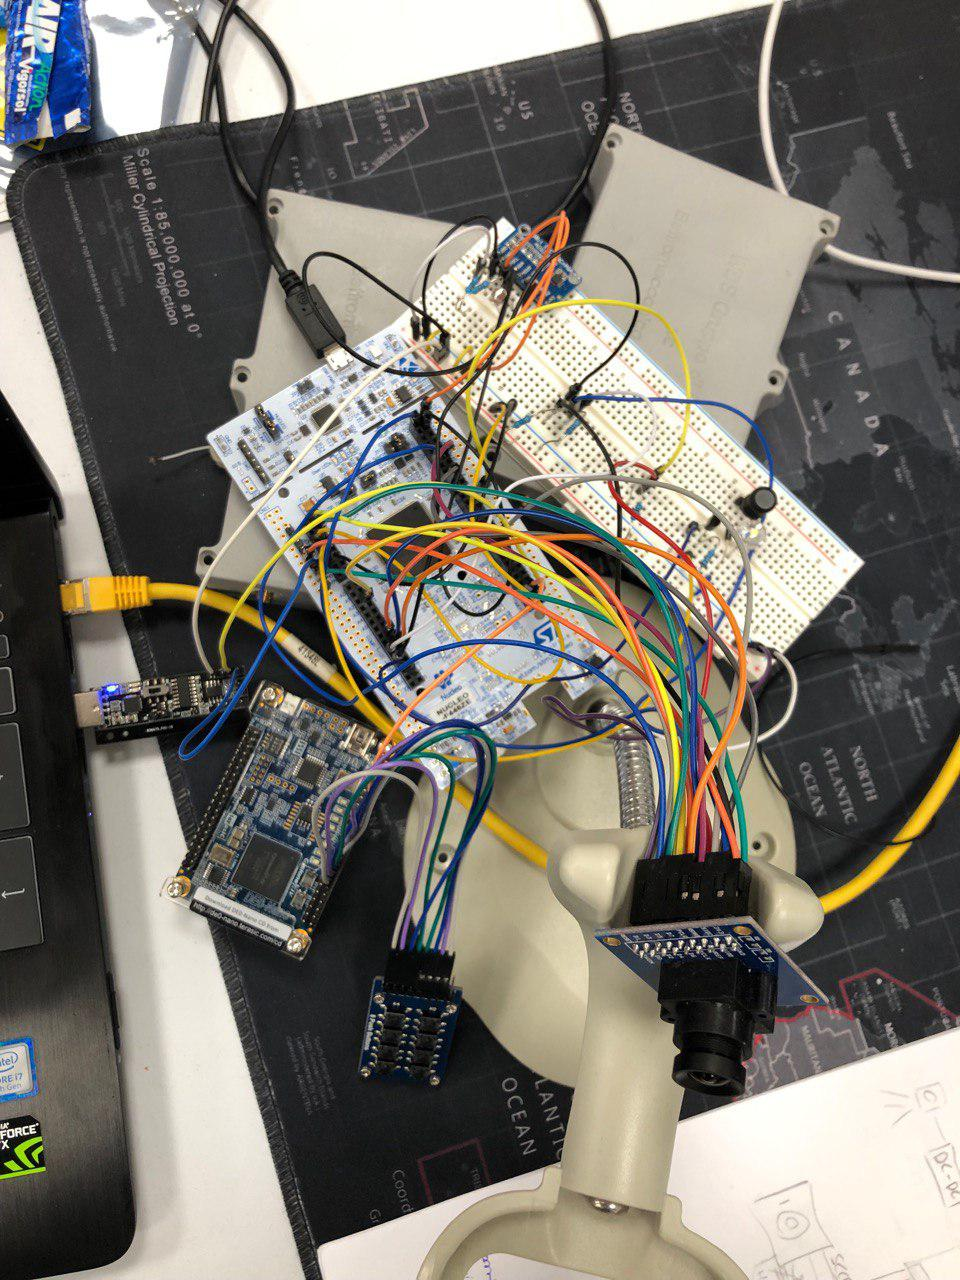
\includegraphics[scale=.4]{Immagini/02}
\label{02}
\caption{Real system}
\end{figure} % Introduction
\section{Analog to digital conversion}
The analog to digital conversion aims at reading the luminance of the room, sending the sample to microcontroller. The input channel is feed by the voltage passing through a photoresistor. After having measured that voltage in condition of both full and absence of light, the dynamics has approximated at range [0.5 - 3.0] Volt.
\newline
The chip is ultra-small, low-Power, 16-Bit analog-to-digital converter with internal reference, provided by Texas Instrument at 3.50\$.
The microcontroller drives it by means of an I2C interface.
\begin{figure}[H]
\centering
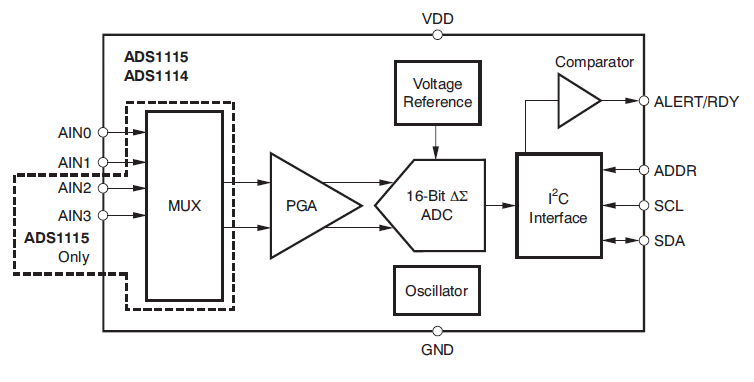
\includegraphics[scale=.7]{Immagini/06}
\label{06}
\caption{A2D internal architecture, from datasheet}
\end{figure}
The chip operates either in continuous conversion mode or a single-shot mode that automatically powers down after a conversion and greatly reduces current consumption during idle periods. I decided to work in the single shot one, sending the command directly from the microcontroller. 
\newline
\newline
In general, to write and read 4 bytes must be sent, the string is composed of the \textbf{slave address} (0x48), the \textbf{register address}, and then in the big-endian format 2 bytes of data. Due to the fact I choose to operate in single shot mode, I have to send every time the command, so the protocol gets as follows: write 4 bytes (including the command), write the slave address and the register address containing the converted data and read 2 byte from it.
\begin{table}[H]
\centering
\begin{tabular}{p{0.5\textwidth}p{0.4\textwidth}}

\textbf{Bit(s) name}&\textbf{Description}\\ \hline
Command & Begin conversion (automatically cleared when completed) \\ 
Input multiplexer configuration & Channel P: In0, Channel N: In1 (physically grounded on breadboard)\\ 
Programmable gain amplifier configuration & $\pm 2.048V$\\
Device operating mode & Power-down single shot mode\\
Data rate & 8 sample per second \\
Comparator mode & not used \\
Comparator polarity & not used \\
Latching comparator & not used \\ \hline
\end{tabular}
\caption{A2D configuration}
\end{table}

\begin{figure}[H]
\centering
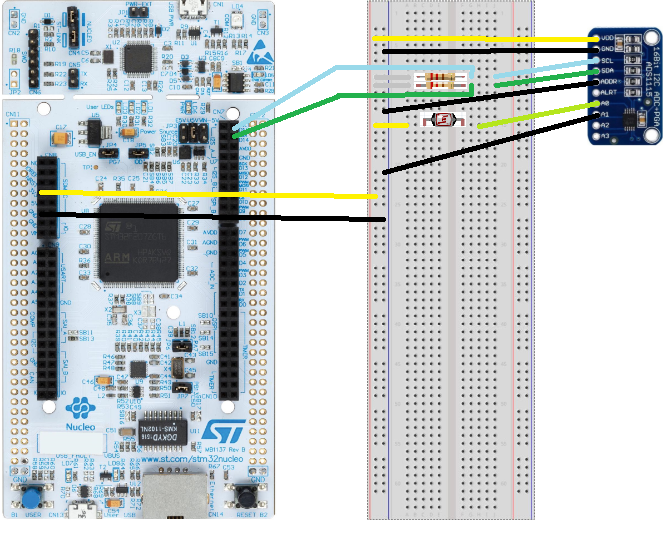
\includegraphics{Immagini/07}
\label{07}
\caption{Connection between MCU and A2D}
\end{figure}

\begin{table}[H]
\centering
\begin{tabular}{p{0.2\textwidth}p{0.4\textwidth}p{0.2\textwidth}}

\textbf{GPIO}&\textbf{Morpho Connector}&\textbf{Description}\\ \hline
PB8 & D15 & I2C1\_SCL\\ 
PB9 & D14 & I2C1\_SDA\\ 
\hline
\end{tabular}
\caption{A2D: GPIOs involved}
\end{table}

\begin{figure}[H]
\centering
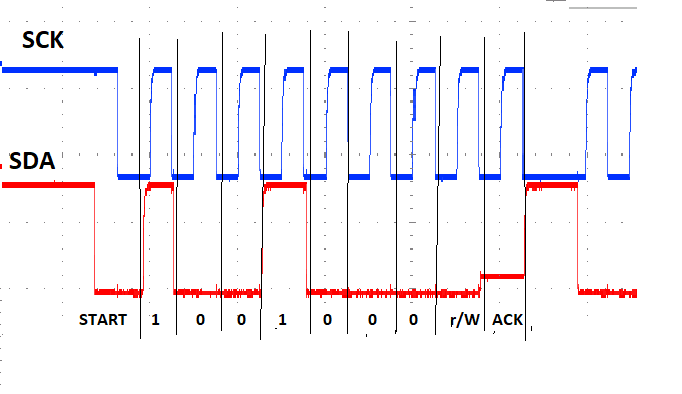
\includegraphics[scale=.7]{Immagini/09}
\label{09}
\caption{Starting an interrogation sending as first byte the slave address of A2D (0x48)}
\end{figure}
 % Analog to digital conversion
\section{Peripheral programming}

 % Peripheral programming
\section{Power management}
Any commercial camera integrates a flash light, which is turned on in leakage of adequate luminance. I have tried to emulate that behaviour using an high emittance LED. I choose a component able to emit a very cold light: it should be fed with 100 mA at 3V. Having defined the load, then I had to chose the input voltage between two possibilities: 3.3 and 5 volts, both of them directly generated by microcontroller and accessible by means of its own morpho connectors. I thought that the former was too close to the desired output, making the implementation of a converter totally useless. So I decided for 5V as input. Due to the fact that I need of a lower voltage, the straightforward architecture is the Bulk one, whose characteristic is
\begin{equation*}
V_{out} = \dfrac{T_{on}V_{in}}{T_{on}+T_{off}} = \delta V_{in}
\end{equation*}
Another, maybe the most important, feature of a switching regulator is the duty cycle used to drive the NPN transistor's base terminal. First of all I adopted a reasonable period $T = T_{on} + T_{off}$. One of the timer on microcontroller is involved in generating the square wave. It's connected to the Advanced Peripheral Bus (APB) which is synchronized with a clock of 16 Mhz. The timer prescaler has been choosen at 160, so each tick is sensed each 10 $\mu s$. Selecting a period of 100 ticks, the overall period $T$ gets $1 ms$, making any consideration about duty cycle easier. However setting duty cycle isn't so simple, something cannot be taken out from a simple equation.
\begin{figure}[H]
\centering
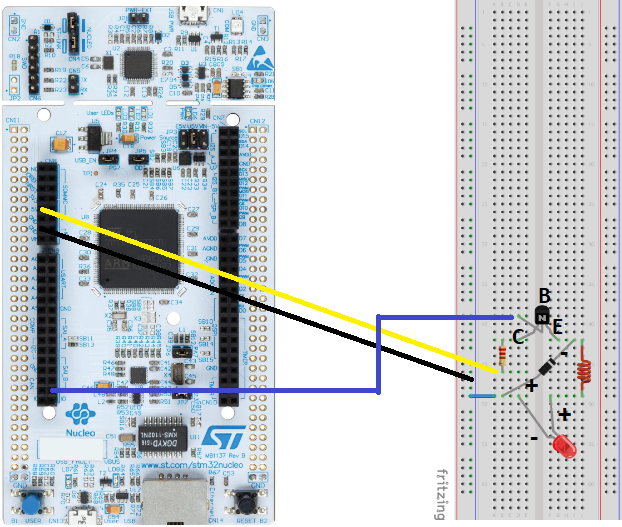
\includegraphics{Immagini/13}
\label{13}
\caption{Connection between MCU and Buck circuit}
\end{figure}

\begin{table}[H]
\centering
\begin{tabular}{p{0.2\textwidth}p{0.4\textwidth}p{0.2\textwidth}}

\textbf{GPIO}&\textbf{Morpho Connector}&\textbf{Description}\\ \hline
PF9 & D63 & TIM14\_CH1 (PWM)\\ 

\hline
\end{tabular}
\caption{Buck: GPIOs involved}
\end{table}

Before showing measurements captured by oscilloscope, I need to state a couple of things. I put a $1K\Omega$ serially the 5V pin in order to avoid overfeeding. It's useless but I was afraid of burning some component: MCU, A2D, camera, resistors, inductor\dots since all of them were connected somehow. Then, few words about the inductor: in the circuit I put $470\mu H$. But, due to the length of $T_{on}$ ($750\mu s$) I would need a much higher one to do not enter in Discontinuos Current Mode. I choose that because it is the biggest I own and have immediate availability. However, everything works and waveforms among the nodes of the circuit seems  to have a compliant shape.

\begin{figure}[H]
\centering
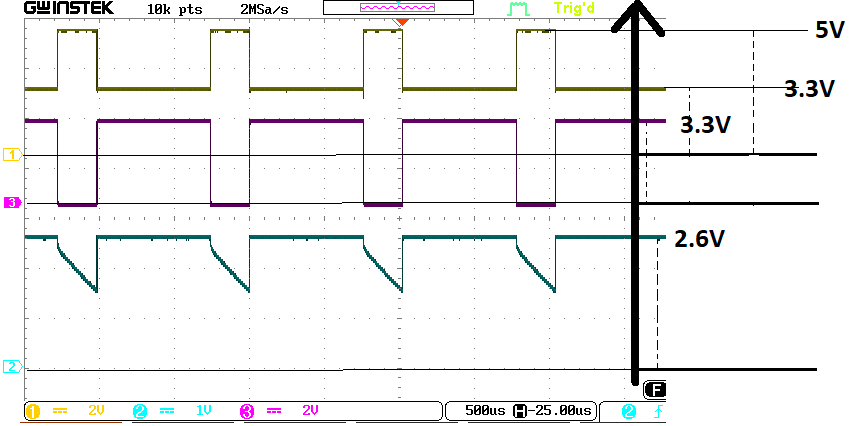
\includegraphics[scale=.7]{Immagini/12}
\label{12}
\caption{From top to bottom: $V_{in}; PWM signal; V_{out}$}
\end{figure}

\begin{figure}[H]
\centering
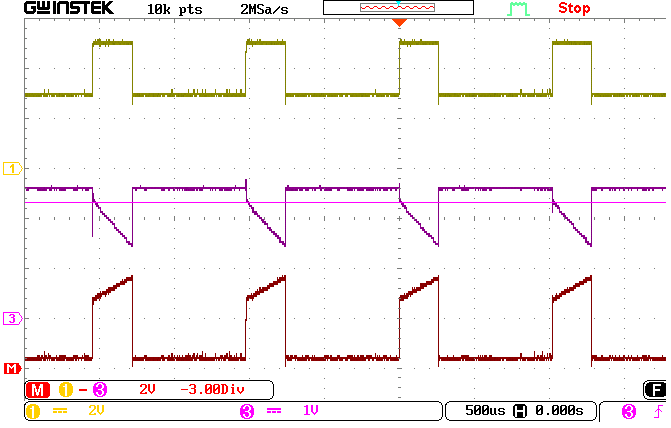
\includegraphics[scale=.8]{Immagini/14}
\label{12}
\caption{From top to bottom: $V_{in}$; $V_A$ of the node where are emitter  diode's cathode and one inductor pin; $V_{out}$, $V_{in}-V_{A}$}
\end{figure}
 % Power management
\section{Programmable logic device}

The behaviour that I tried to emulate by means of the FPGA consists in reading the status of a group of bottoms and send them to the microcontroller via single wire communication protocol: UART. So, the overall architecture is composed of two main parts:
\begin{itemize}
\item The logic of interface for the keyboard
\item UART peripheral VHDL-based (only TX channel). It will be described in the next section
\end{itemize}

\begin{figure}[H]
\centering
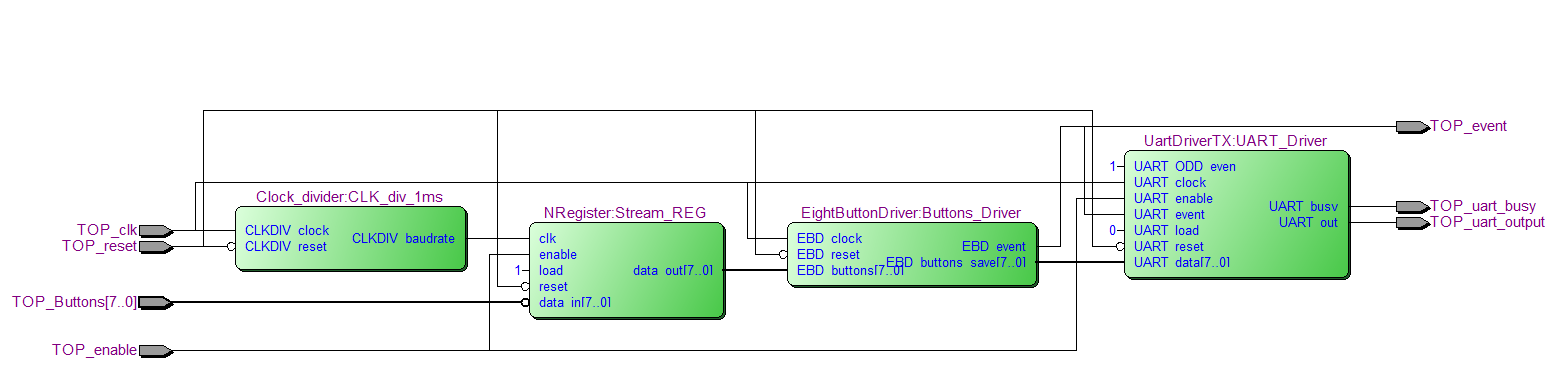
\includegraphics[scale=.5]{Immagini/15}
\label{15}
\caption{Top level entity view}
\end{figure}

Clock is internally generated by the FPGA at 50 MHz, however in some point of the architecture I needed to slow down. The clock feeding the output shift register within UART peripheral block runs at 115400 bit/s around. Another clock divider is used to sample buttons each 1 ms. During my tests, I noticed that the architecture worked well in simulation, but scoping the UART output with an oscilloscope probe I saw the mess. This totally uncorrect behaviour was given by the fact that button are mechanical objects generating a bouncing signal when pushed. So I measured the duration of these oscillations, leading me at the conclusion of implementing a "debouncing logic", in my project composed of a register and a clock divisor, the ones are shown in the top level entity view. The input signals got stable after some hundreds of $\mu s$, until $800 \mu s$ in some cases. That's the reason why I perform input sampling each one millisecond. I'm sure that in this interval oscillations expire.
\newline
\newline
Clock dividers I implemented are both fed by the 50 Mhz clock. Internally the output of a counter is compared with the one contained within an hardwired register. The comparator performs the equality checking operation. Every time comparison gets true, the counter is reset in next cycle. 
 The output of clock divider is the one of the comparator; in such a way the resulting waveform is a train of pulses having the desired baudrate.
 \begin{figure}[H]
\centering
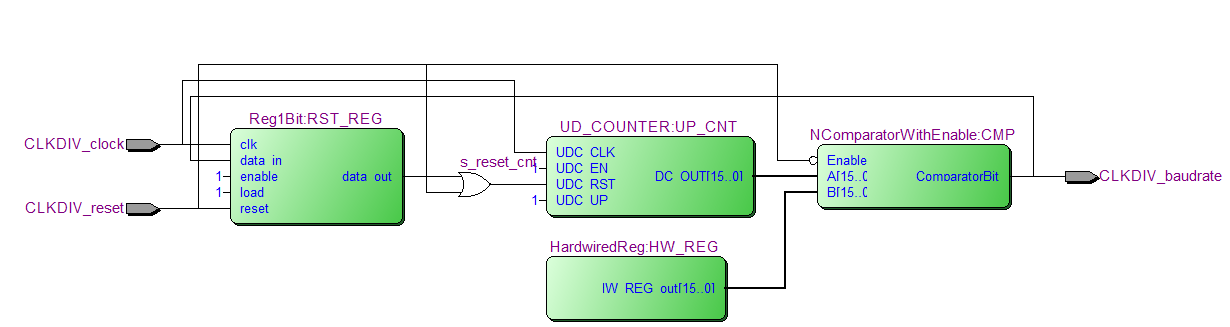
\includegraphics[scale=.6]{Immagini/17}
\label{17}
\caption{Clock divider architecture}
\end{figure}
 \begin{figure}[H]
\centering
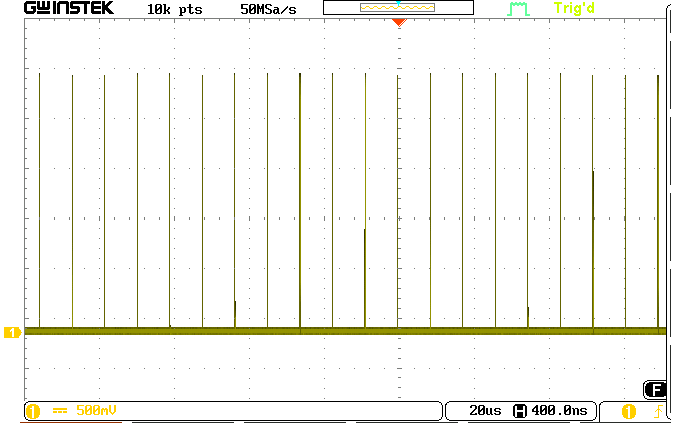
\includegraphics{Immagini/16}
\label{16}
\caption{Clock divider output within UART peripheral. Time between two consecutive pulses is $9 \mu s$, leading a baudrate of 115200 bit/s. The hardwired value is 434, from the round division between 50Mhz and 115200 Hz}
\end{figure}

The eight buttons driver just simply recognizes when a button has been pushed and generates an "event", then sent to the UART peripheral to start the transfer. Two registers are on the output, one for buttons, one for the event bit.
\newline
\newline
I'm going to talk about UART peripheral implementation in the next section, dedicated to \textbf{Interconnection protocol}. Another VHDL component, that is not integrated here, is the memory controller for the SDRAM laid on the Altera board; the last section \textbf{Memory management} is dedicated to it and some comparisons between waveform simulation and real required access protocol will be shown.

 \begin{figure}[H]
\centering
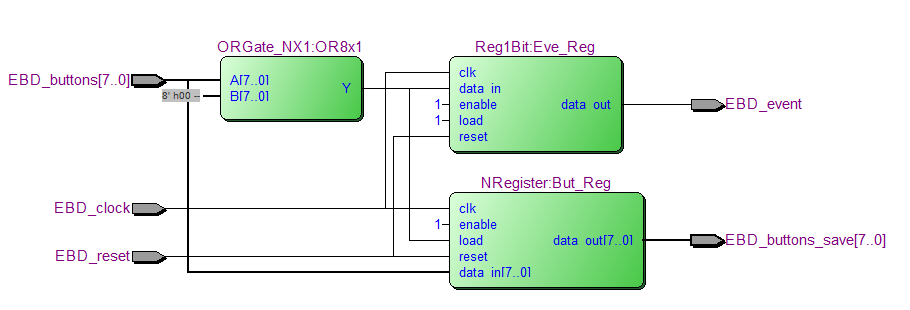
\includegraphics[scale=.8]{Immagini/18}
\label{18}
\caption{Eight button driver architecture}
\end{figure}

\begin{table}[H]
\centering
\begin{tabular}{p{0.3\textwidth}p{0.2\textwidth}p{0.3\textwidth}}

\textbf{Node name}&\textbf{Direction}&\textbf{Location}\\ \hline
TOP\_reset & Input & J15 (Push Button[0])\\
TOP\_enable& Input & M1 (DIP\_switch[0])\\
TOP\_clk	&Input & R8 (Internal clock source 50 Mhz)\\
TOP\_buttons[0]	& Input & D5 (GPIO\_09)\\ 
TOP\_buttons[1]	& Input & A6 (GPIO\_011)\\ 
TOP\_buttons[2]	& Input & D6 (GPIO\_013)\\ 
TOP\_buttons[3]	& Input & C6 (GPIO\_015)\\ 
TOP\_buttons[4]	& Input & E6 (GPIO\_017)\\ 
TOP\_buttons[5]	& Input & D8 (GPIO\_019)\\ 
TOP\_buttons[6]	& Input & F8 (GPIO\_021)\\ 
TOP\_buttons[7]	& Input & E9 (GPIO\_023)\\ 
TOP\_uart\_output & Output & D3 (GPIO\_00)\\
TOP\_uart\_busy	  & Output & C3 (GPIO\_01), not used, just for debugging\\
TOP\_event		& Output	& A3 (GPIO\_03), not used, just for debugging\\
\hline
\end{tabular}
\caption{FPGA pin assignment}
\end{table}

\begin{figure}[H]
\centering
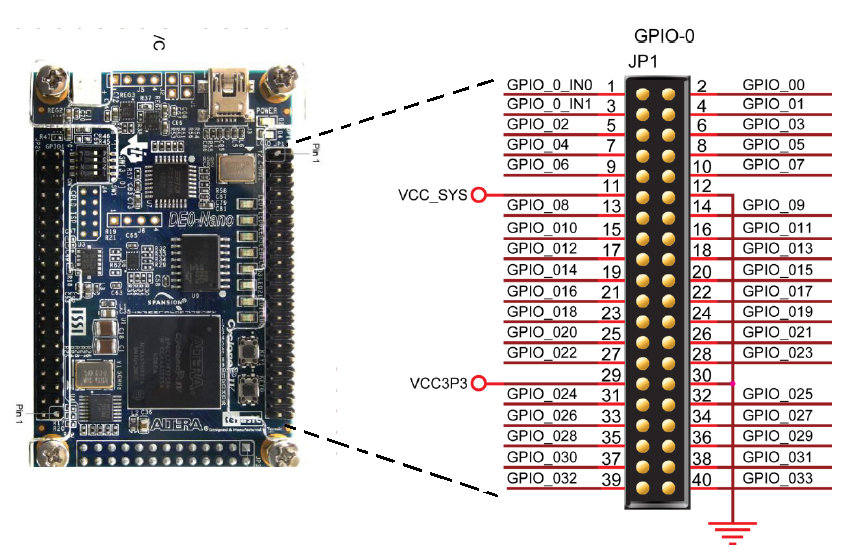
\includegraphics[scale=.8]{Immagini/19}
\label{19}
\caption{Altera DE0 Nano GPIO pinout}
\end{figure} % Programmable logic device
\section{Interconnection protocol}
The target interconncection protocol is the UART, which is in charged to allow communication from the FPGA and microcontroller. Main settings regard the baudrate (115200 bit/s), the length of data (8), the parity ODD bit and one stop bit. Considering also the start, the UART peripheral gets busy for 11 cycles.
\newline
\newline
The clock divider generates a train of pulses at 115200 Hz. I talked about clock divider implementation in the previous section. A module called UART synchronizer takes the peripheral busy for 11 cycles. This component receives as input that train of pulses, rather than the FPGA's clock. Conceptually, the synchronizer has a structure very similar to the one of clock divider: a counter, an hardwired register and a comparator. The synchronizer task is to send the shift command to the shift register storing the data to be sent via serial protocol. So, instead of using an equality comparator, I put here an inequality one. Until the value of the counter is less or equal than the value in the hardwired register (10) the UART is being busy. Another difference regards the counter resetting. The UART logic works only in response to an external action, like an interrupt; the train of pulses is generated periodically regardless of buttons status instead. I mean that, after those 11 cycles, the shift command gets disabled but counter is counting up without stopping. A classic counter gets overflow when reaches the all 1s string, turning the peripheral busy in absence of event ($0 \leq 10$). A \textit{saturation counter} keeps at all 1s and has reset to 0 only when an external event has triggered.

\begin{figure}[H]
\centering
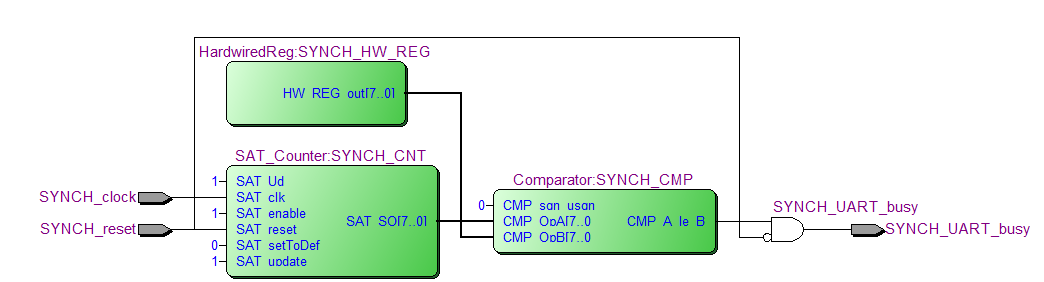
\includegraphics[scale=.8]{Immagini/20}
\label{20}
\caption{UART synchronizer architecture}
\end{figure}

I think that a couple of words should be spent on the shift register, which is named UART\_Fifo. It is a common shift register parallel input serial output. However, it is between two frequency domains, the 50 Mhz and the 115Khz. The coming data is loaded with former domain, shifting has performed at the latter. The clock signal going in input to each flip flop is the result of an OR between the 115Khz clock and the load command travelling at 50Mhz. Then, a few combinational logic drives multiplexers in order to perform operations of KEEPING, SHIFTING and LOADING.
\newline
\newline
To prove the correct behaviour of my UART module, before I plotted the output signal onto the oscilloscope, then I used a software serial terminal like Hterm using the same settings I listed above; the picture shows one of eight buttons forming the keyboard pushed one at a time.

\begin{figure}[H]
\centering
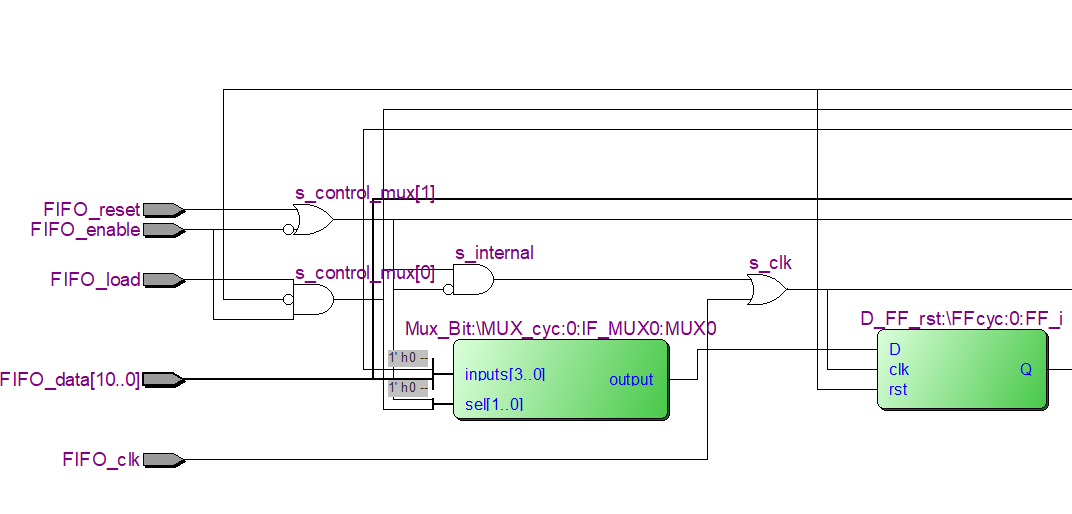
\includegraphics[scale=.7]{Immagini/23}
\label{23}
\caption{UART Fifo architecture: combinational logic to drive multiplexers and FF clock}
\end{figure}

\begin{figure}[H]
\centering
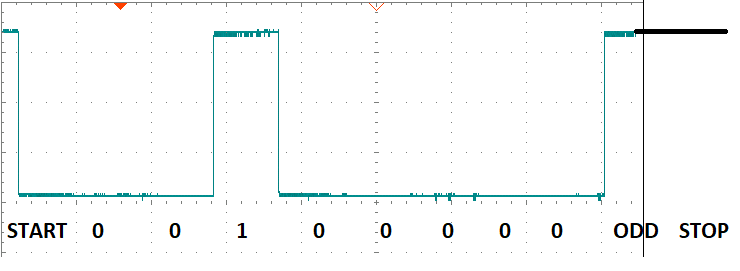
\includegraphics[scale=.9]{Immagini/21}
\label{21}
\caption{UART output on oscilloscope (10 $\mu s$/div)}
\end{figure}

\begin{figure}[H]
\centering
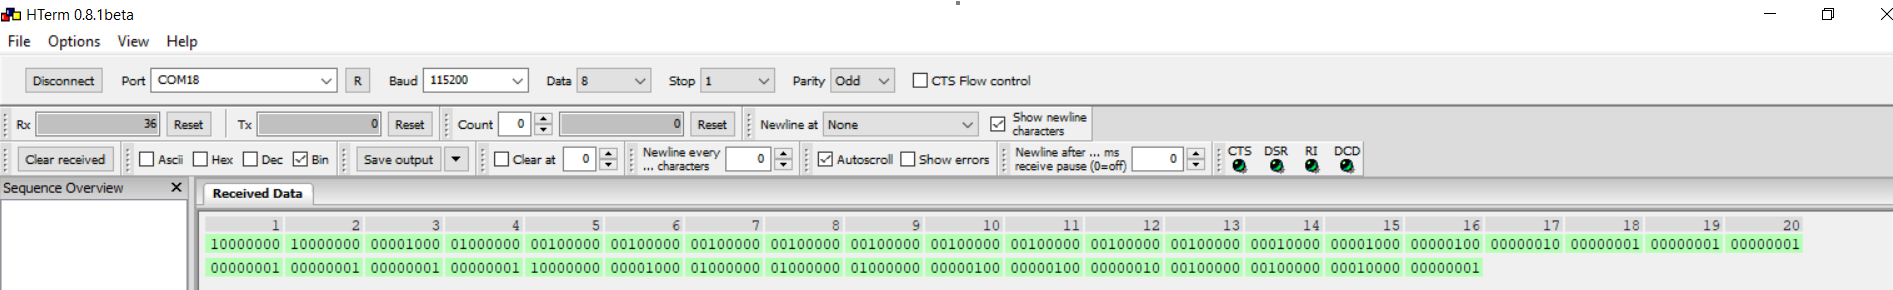
\includegraphics[scale=.4]{Immagini/22}
\label{22}
\caption{UART output on HTerm (serial terminal)}
\end{figure}

\begin{figure}[H]
\centering
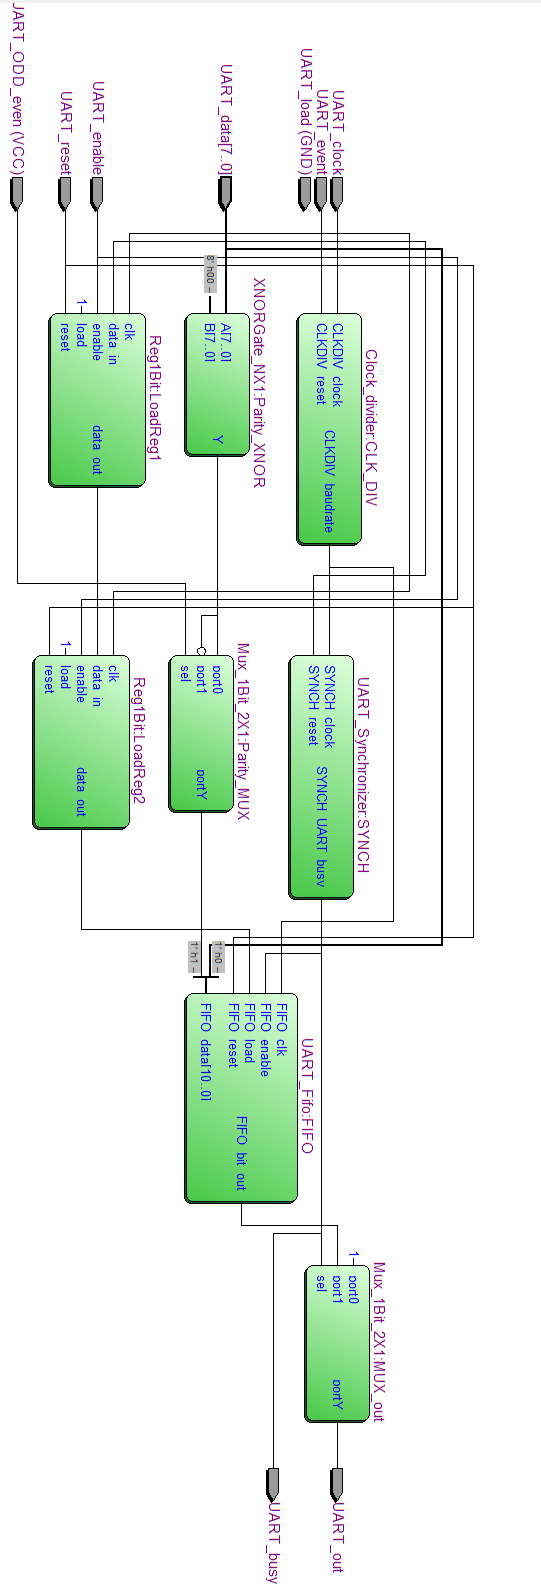
\includegraphics[scale=.7]{Immagini/24}
\label{24}
\caption{UART module architecture}
\end{figure} % Interconnection protocol
\section{Memory management}

My goal for this part was to store the data read from buttons driver in a single memory location and then read it plotting tha value by means of the array of leds on the Altera board. First of all I had to implement the memory controller to run access protocols, but in any case I no reached to synchronize correctly the manager and the memory. In the end, my memory controller just emulates the access protocols, satisfying the waveform shapes for each clock cycles; however any consideration about access time or similar have been discharged.
\newline
Two words about the target memory. It's a 256 Mbits SDRAM provided by ISSI. It's fully synchronous, offers the possibility to do burst transfers, does auto-refreshing, allows programmable CAS latency and so on.
\newline
\newline
As first, I needed to know how FPGA is interfaced with SDRAM.
\begin{figure}[H]
\centering
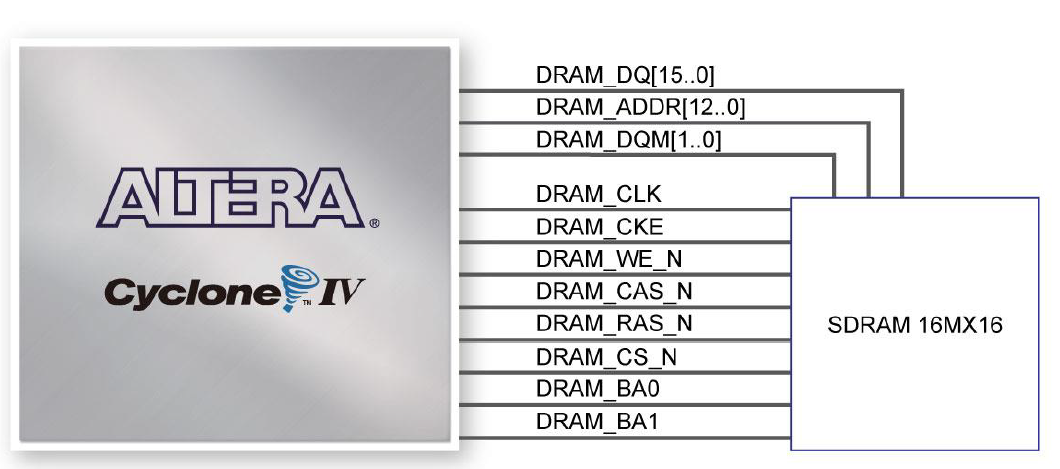
\includegraphics[scale=.7]{Immagini/25}
\label{25}
\caption{Connections between FPGA chip and SDRAM}
\end{figure}

There are 13 bits of address $Ax$ and 16 bits input/output for data. The SDRAM is composed of 4 banks 8192 size each; to select one of them 2 input bits called Bank Select Address are used. Then the clock and clock enable are inputs as well. Moreover, there are the chip select, the write enable, the row address strobe and the column address strobe, all of them active low. This SDRAM offers possibility to mask the output, driving the 2 Data Masked bits, for the high and low parts respectively.
\newline
\newline
My module is a classic finite state machine, where each step is generated on the rising edge of the clock. The FSM is composed of 20 states. Looking at the datasheet, the state diagram is more complex so I decided to build it implementing the basic operations: the initialization, the programming,  the request of a read the the request of a write. In between, memory expects to be precharged and refreshed. What I'm going to show in this section is the comparison between waveforms I'm able to generate and what is shown in the datasheet.
\newpage


\begin{lstlisting}[caption=VHDL entity of memory manager, language=VHDL]
entity MemoryInterface is
	port(
		MI_buttons : in std_logic_vector(7 downto 0);
		MI_clk	 : in std_logic;
		MI_reset : in std_logic;
		MI_enable : in std_logic;
		MI_RW : in std_logic; -- external event, no event reading, event writing
		MI_action : in std_logic; -- active low
		MI_address : in std_logic_vector(14 downto 0);
		
--		real interface
		
		MI_address_9_0 : out std_logic_vector(9 downto 0);
		MI_address_10 : out std_logic;
		MI_address_12_11: out std_logic_vector(12 downto 11);
		MI_bank : out std_logic_vector(1 downto 0);
		MI_data : inout std_logic_vector(15 downto 0);
		MI_CAS : out std_logic; -- active low
		MI_RAS : out std_logic; -- active low
		MI_CS : out std_logic; -- active low
		MI_write_enable : out std_logic; -- active low
		MI_clk_enable : out std_logic; -- active high
		MI_memory_clk : out std_logic;
		MI_DQML : out std_logic;
		MI_DQMH : out std_logic
	);
end MemoryInterface;
\end{lstlisting}

\begin{figure}[H]
\centering
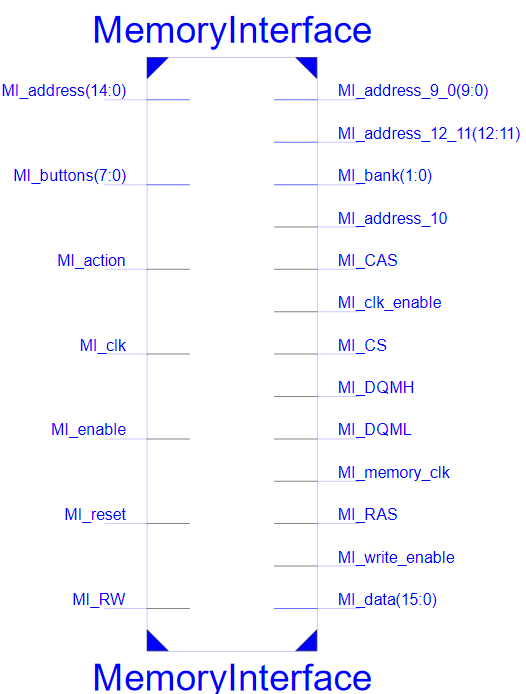
\includegraphics[scale=.6]{Immagini/27}
\label{27}
\caption{Memory interface pinout}
\end{figure}

\begin{figure}[H]
\centering
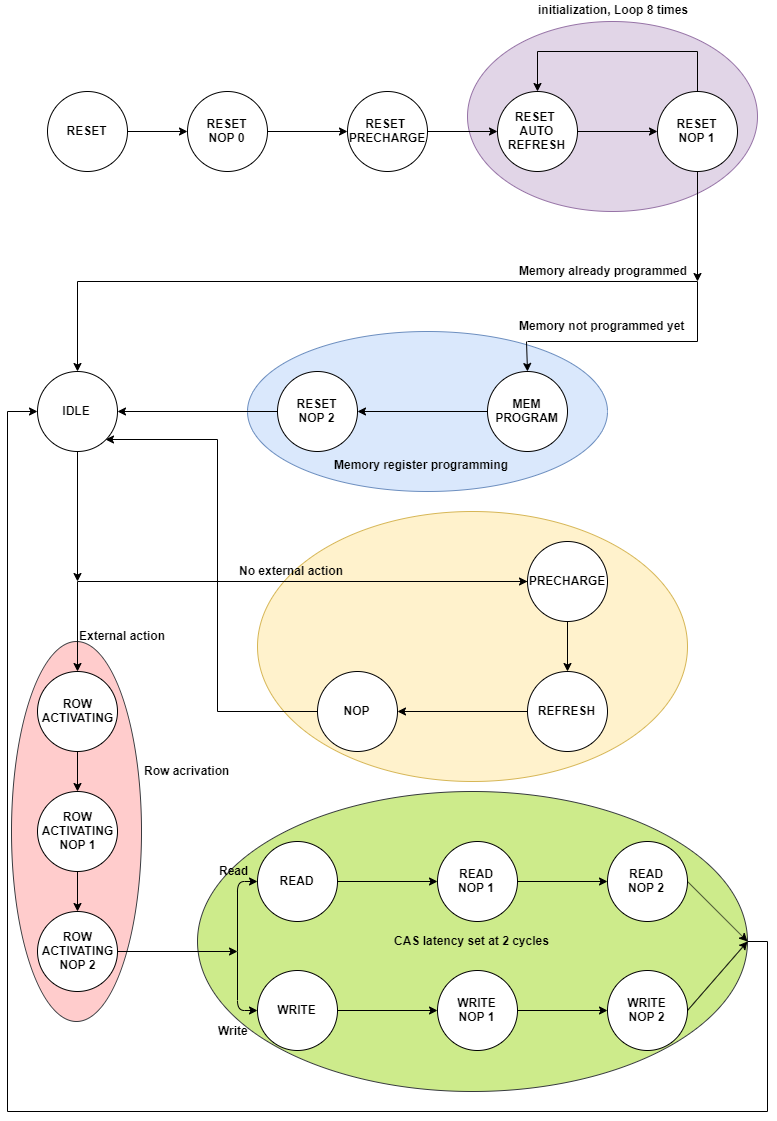
\includegraphics[scale=.6]{Immagini/26}
\label{26}
\caption{Memory controller state diagram}
\end{figure}

\begin{figure}[H]
\centering
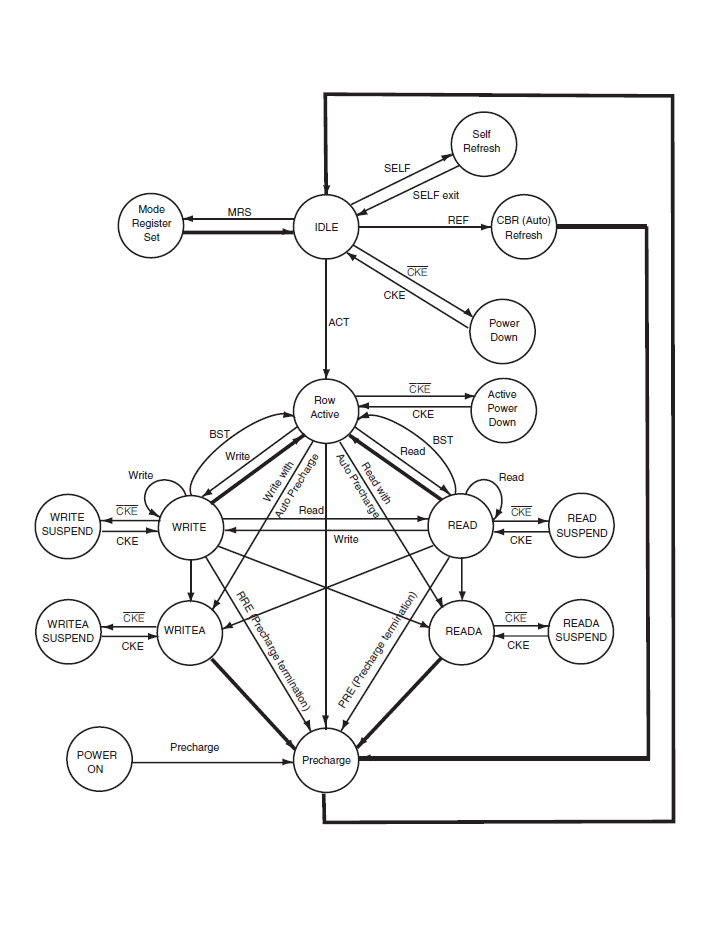
\includegraphics[scale=1.1]{Immagini/34}
\label{26}
\caption{Memory state diagram from datasheet}
\end{figure}

When reset pin has activated, the SDRAM is once precharged, then for 8 times alternates a cycle of refreshing and one cycle of NOP. The bit 10 of the address, provides memory information about refreshing. If it's '1' all banks are refreshed, otherwise only the one is indicated by MI\_bank bits. After initialization, the manager should be program the control register of the memory, which provides some information such as: burst length (1), burst type (sequential), CAS latency (2) and write burst mode (single location access). The state memory load register follows the end of initialization loop.

\begin{figure}[H]
\centering
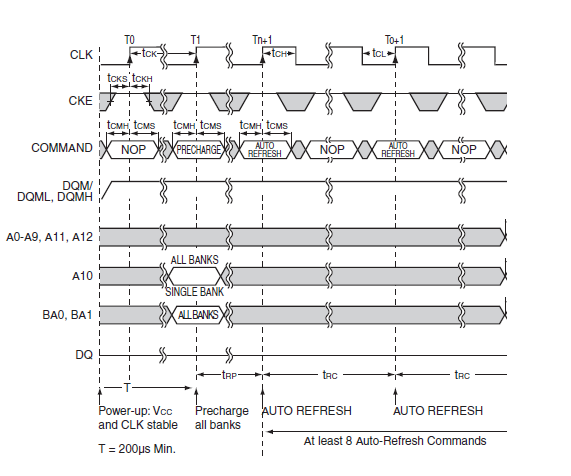
\includegraphics{Immagini/29}
\label{29}
\caption{Initialization: datasheet}
\end{figure}

\begin{figure}[H]
\centering
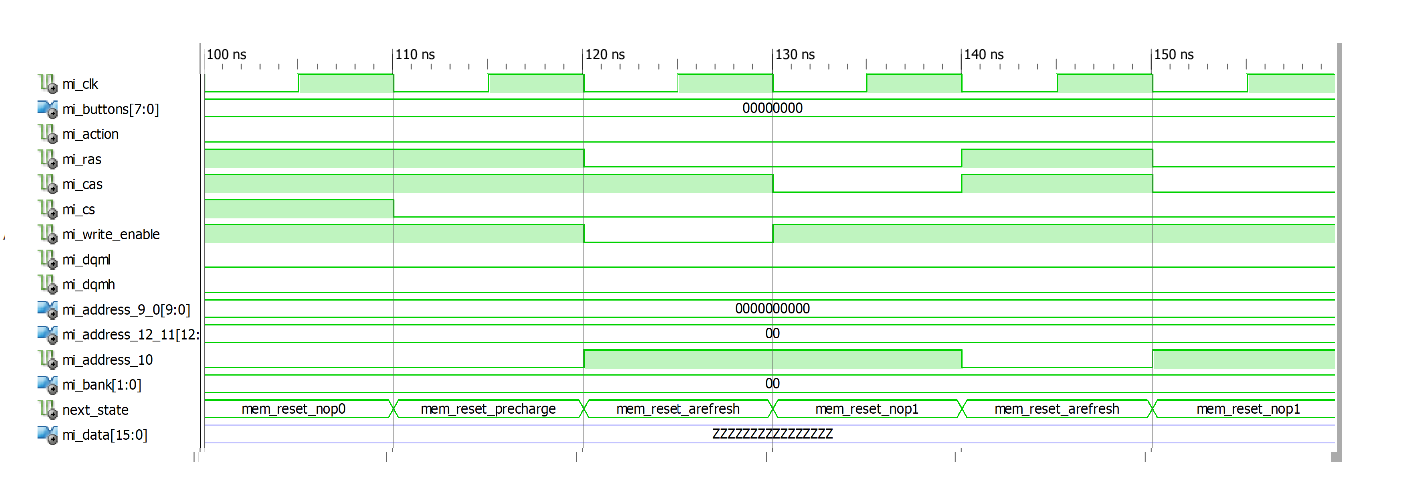
\includegraphics[scale=.5]{Immagini/28}
\label{28}
\caption{Initialization: simulation}
\end{figure}
\newpage
From the idle state, the controller detects that an action has been driven from outside. From idle the state diagram moves toward the activation on the target row, which is passed on address pins and recognized by activating the row address strobe. After two cycles, memory controller sends the data and the column address, activating the CAS in the meantime. Since CAS latency has been set to 2 cycles, memory requires two NOP cycles to accomplish the operation. Small note for the reader: both read and write can be performed with or without auto-precharging, depending on the logic value on the 10th bit of address. Due to the fact that, in datasheet, the time diagrams of write both with auto precharge and without are totally equal, while read diagrams differ from the explicit presence of that (how we will see next), I guess that write with auto precharging diagram is wrong. Precharging command should not be sent from memory controller.

\begin{figure}[H]
\centering
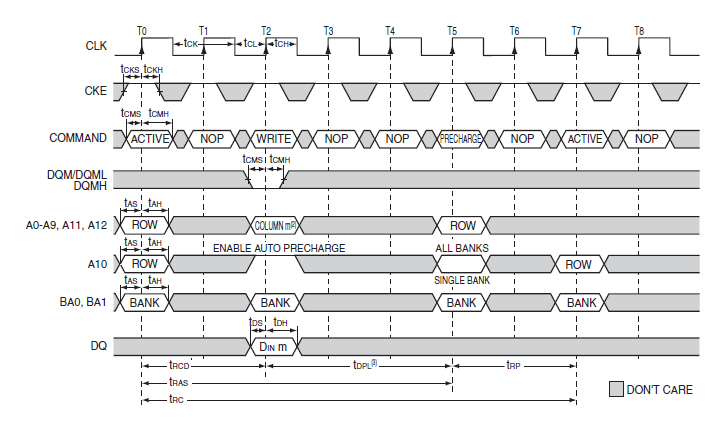
\includegraphics[scale=.9]{Immagini/31}
\label{31}
\caption{Write: datasheet}
\end{figure}

\begin{figure}[H]
\centering
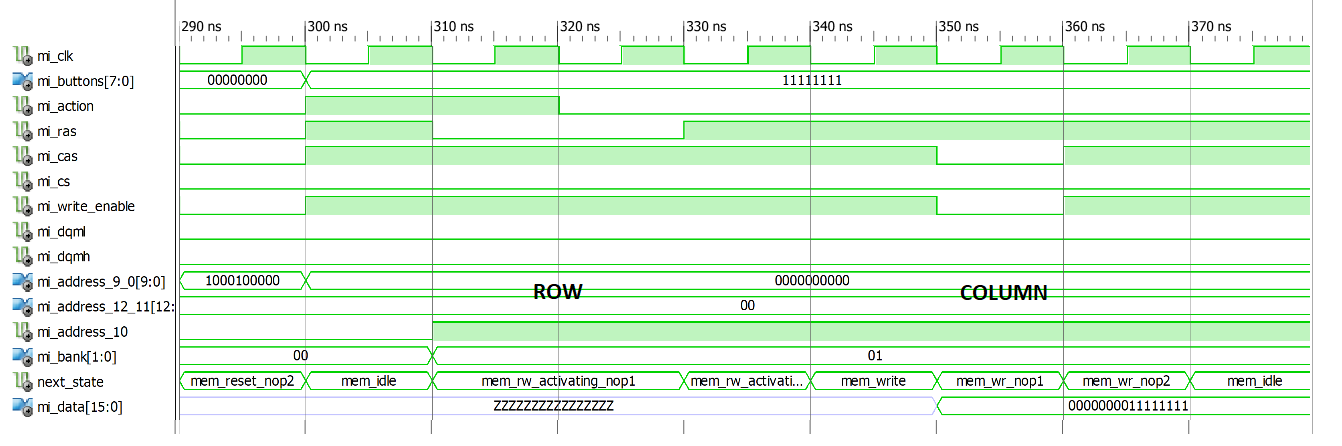
\includegraphics[scale=.5]{Immagini/30}
\label{30}
\caption{Write: simulation}
\end{figure}

\newpage

As you can see from the datasheet diagram, when the operation has been set with autoprecharging, that command is not sent but automatically performed by memory internally. 

\begin{figure}[H]
\centering
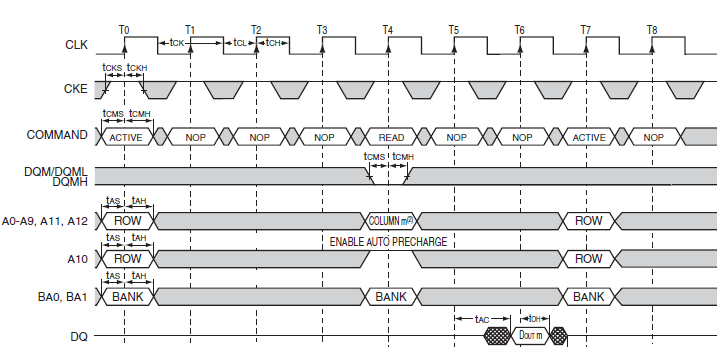
\includegraphics[scale=.9]{Immagini/33}
\label{33}
\caption{Read: datasheet}
\end{figure}

\begin{figure}[H]
\centering
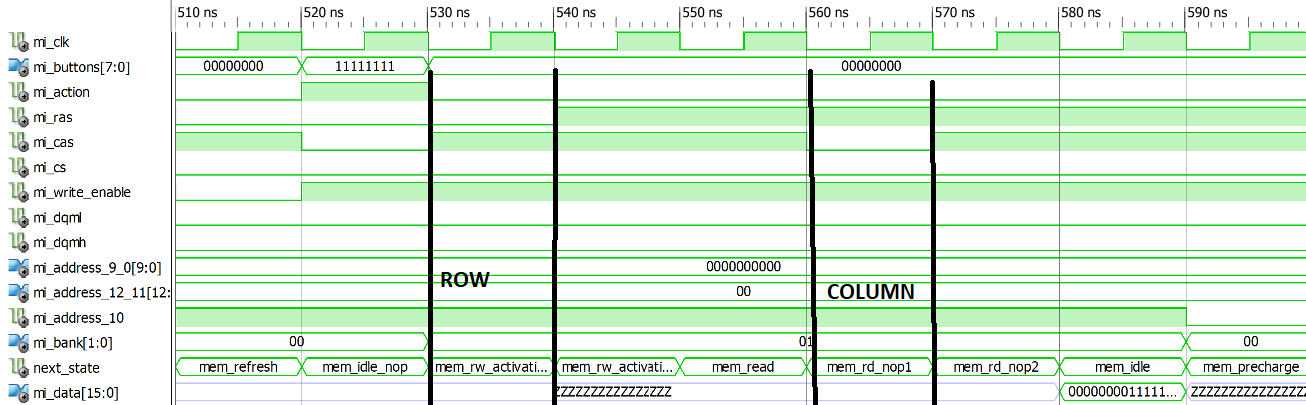
\includegraphics[scale=.5]{Immagini/32}
\label{32}
\caption{Read: simulation}
\end{figure}

\begin{figure}[H]
\centering
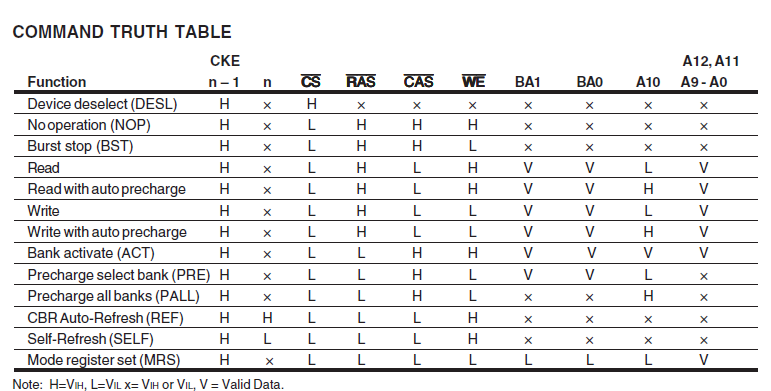
\includegraphics[scale=.8]{Immagini/35}
\label{35}
\caption{Main commands format}
\end{figure} % Memory management
\section{Conclusion}

I started working on this system on 1st of October and the development ended on 12nd of November, for a global amount of 240 hours of workload.
I'd like to highlight the main difficulties I found and how I fixed them, but it's something I'm going to do during the presentation of the project.
\newline
Approximately, considering all hardware I bought, not what I burnt, this kind of system costs 150 euros. Anyway, that price will be lower for sure. If I wanted to draw a real circuit PCB, for sure I would use the embedded ADC of the microcontroller; moreover I would choose a microcontroller having a smaller number of pins, so removing a lot of peripherals that I didn't initialize; then, the implementation by PCB would make the breadboard useless.
\newline
Another thing that I could improve is the Python script to re-build images. Currently it just generates black and white pictures, a better code would fill them by colors.
\newline
A further step consists in resizing components in Buck circuit, in order to optimize consumptions. Some other pictures follow and end the report.
\begin{figure}[H]
\centering
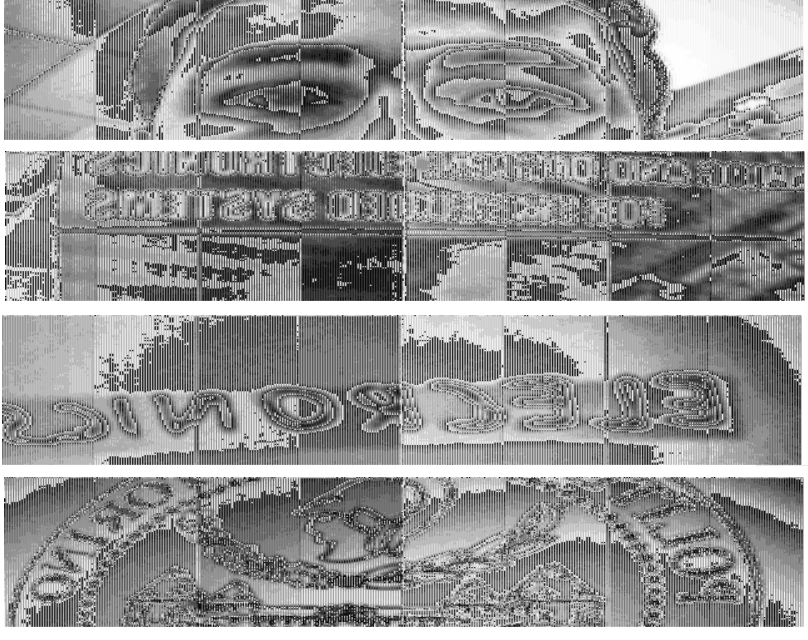
\includegraphics[scale=.9]{Immagini/test99}
\label{04}
\end{figure}

 % Conclusion

\end{document}
